\documentclass[xcolor=dvipsnames,table]{beamer}

\usepackage{latexsym}
\usepackage[utf8]{inputenc}
\usepackage[brazil]{babel}
\usepackage{amssymb}
\usepackage{amsmath}
\usepackage{stmaryrd}
\usepackage{fancybox}
\usepackage{datetime}
\usepackage[T1]{fontenc}
\usepackage{graphicx}
\usepackage{graphics}
\usepackage{url}
\usepackage{algorithmic}
\usepackage{algorithm}
\usepackage{acronym}
\usepackage{array}

\newtheorem{definicao}{Definio}
\newcommand{\tab}{\hspace*{2em}}

\mode<presentation>
{
  \definecolor{colortexto}{RGB}{0,0,0}
 
  \setbeamertemplate{background canvas}[vertical shading][ bottom=white!10,top=white!10]
  \setbeamercolor{normal text}{fg=colortexto} 

  \usetheme{Warsaw}
}

\title{Máquina de Turing} 

\author{
  Esdras Lins Bispo Jr. \\ \url{bispojr@ufg.br}
  } 
 \institute{
  Teoria da Computação \\Bacharelado em Ciência da Computação}
\date{\textbf{02 de abril de 2018} }

\logo{
\includegraphics[width=1cm]{images/ufgJataiLogo.png}}

\begin{document}

	\begin{frame}
		\titlepage
	\end{frame}

	\AtBeginSection{
		\begin{frame}{Sumário}%[allowframebreaks]{Sumário}
    		\tableofcontents[currentsection]
    		%\tableofcontents[currentsection, hideothersubsections]
		\end{frame}
	}

	\begin{frame}{Plano de Aula}
		\tableofcontents
		%\tableofcontents[hideallsubsections]
	\end{frame}
	
	
%------------------------------------------
\section{Pensamento}
\begin{frame}{Pensamento}
	\begin{center}
		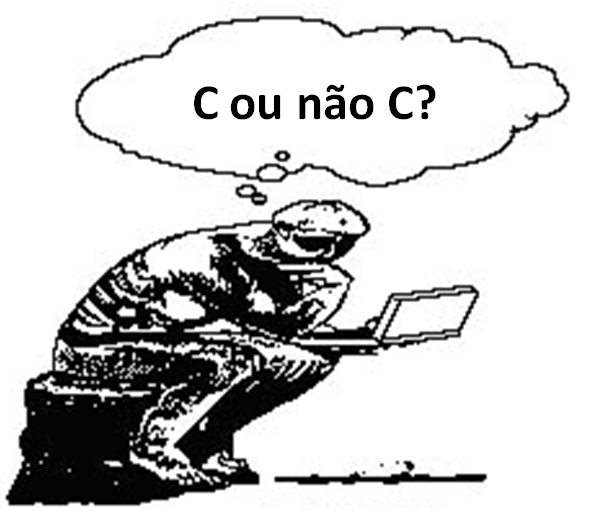
\includegraphics[width=7cm]{images/pensamento.png}
	\end{center}
\end{frame}

\begin{frame}{Pensamento}
	\begin{columns}
		\column{.4\textwidth}  		
		\begin{center}
			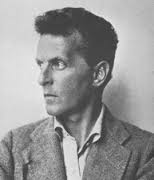
\includegraphics[height=.5\textheight]{images/wittgenstein.jpg}
		\end{center}
		\column{.6\textwidth}  		
		\begin{block}{Frase}
			\begin{center}
				{\large Os limites do meu conhecimento são os limites do meu mundo.}
			\end{center}
		\end{block}		  		
		\begin{block}{Quem?}
			\begin{center}
				{\bf Ludwig Wittgenstein (1889-1951)} \\ Filósofo austríaco.
			\end{center}
		\end{block}
	\end{columns}
\end{frame}
%------------------------------------------
\section{Introdução}
\subsection{O que é Teoria da Computação?}
\begin{frame}{O que é Teoria da Computação?}
	Pode ser dividida em três grandes áreas:
	\begin{itemize}
		\item Teoria dos Autômatos;
		\item Teoria da Computabilidade;
		\item Teoria da Complexidade.	
	\end{itemize}\pause
	São interligadas pela pergunta:
	\begin{block}{}
		Quais são as capacidades e limitações fundamentais dos computadores?
	\end{block}
\end{frame}

\begin{frame}{O que é Teoria da Computação?}
	\begin{block}{Teoria dos Autômatos}
		Quais são as definições e propriedades dos modelos matemáticos de computação?
	\end{block} \pause
	\begin{block}{Teoria da Computabilidade}
		O que faz alguns problemas serem solúveis e outros não?		
	\end{block} \pause
	\begin{block}{Teoria da Complexidade}
		O que faz alguns problemas serem computacionalmente difíceis e outros fáceis?
	\end{block}
\end{frame}

\section{Máquina de Turing}
\begin{frame}{Modelos Básicos Computacionais}
	\begin{block}{AFDs, AFNs, e Expressões Regulares}
		\begin{itemize}
			\item Potencialidades: reconhecem linguagens como $({\tt 10} \cup {\tt 1})^*$;
			\item Fragilidades: não reconhecem linguagens como $A = \{ {\tt 0}^n {\tt 1}^n \mbox{ | } n \geq 0 \mbox{ e } n \in \mathbb{N} \}$.
		\end{itemize}
	\end{block} \pause
	\begin{block}{GLCs e Autômatos com Pilha}
		\begin{itemize}
			\item Potencialidades: reconhecem linguagens como $A = \{ {\tt 0}^n {\tt 1}^n \mbox{ | } n \geq 0 \mbox{ e } n \in \mathbb{N} \}$;
			\item Fragilidades: não reconhecem linguagens como $A = \{ {\tt a}^n {\tt b}^n {\tt c}^n\mbox{ | } n \geq 0 \mbox{ e } n \in \mathbb{N} \}$.
		\end{itemize}
	\end{block} \pause
	\begin{alertblock}{}
		Portanto são bem restritos para servir de modelo de computadores de propósito geral.
	\end{alertblock}
\end{frame}

\begin{frame}{Máquinas de Turing (MT)}
	\begin{itemize}
		\item Modelo mais poderoso que GLCs e AFDs; \pause
		\item Turing, 1936; \pause
		\item Características importantes:
		\begin{enumerate}
			\item faz tudo o que um computador real pode fazer;
			\item existem certos problemas que uma MT não pode resolver.
		\end{enumerate}				 
	\end{itemize}
\end{frame}
	
	\begin{frame}{Máquinas de Turing (MT)}
		\begin{center}
			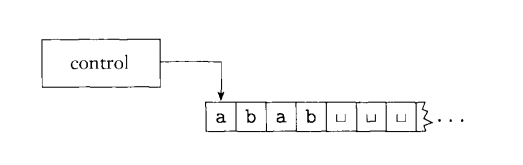
\includegraphics[height=3.5cm]{images/fig31.png}
		\end{center}
	\end{frame}
	
	\begin{frame}{Máquinas de Turing (MT)}
		\begin{block}{Diferenças entre MT e AFDs}
			\begin{itemize}
				\item Uma MT pode tanto escrever sobre a fita quanto ler a partir dela; \pause
				\item A cabeça de leitura-escrita pode mover-se tanto para a esquerda quanto para a direita; \pause
				\item A fita é infinita; \pause
				\item Os estados especiais para rejeitar e aceitar fazem efeito imediatamente.
			\end{itemize}
		\end{block}
	\end{frame}
	
	\begin{frame}{Máquinas de Turing (MT)}
		\begin{block}{Construindo uma MT}
			\begin{center}
				Construir $M_1$ que reconheça a linguagem $B = \{ \omega \# \omega \mbox{ | } \omega \in \{ 0, 1 \}^* \}$.
			\end{center}
		\end{block}
	\end{frame}
	
	\begin{frame}{Máquinas de Turing (MT)}
		\begin{block}{Descrição de $M_1$}
			$M_1 =$ ``Sobre a cadeia de entrada $\omega$:
			\begin{enumerate}
				\item Faça um zigue-zague ao longo da fita checando posições correspondentes de ambos os lados do símbolo $\#$ para verificar se elas contêm o mesmo símbolo. Se elas não contêm, ou se nenhum $\#$ for encontrado, {\it rejeite}. Marque os símbolos à medida que eles são verificados para manter registro de quais símbolos têm correspondência.
				\item Quando todos os símbolos à esquerda do $\#$ tiverem sido marcados, verifique a existência de algum símbolo remanecente à direta do $\#$. Se resta algum símbolo, {\it rejeite}; caso contrário, {\it aceite}.
			\end{enumerate}
		\end{block}
	\end{frame}
	
	\begin{frame}{Máquinas de Turing (MT)}
		\begin{center}
			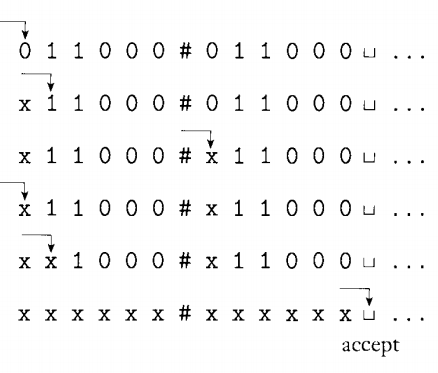
\includegraphics[height=6cm]{images/fig32.png}
		\end{center}
	\end{frame}	
	
	\begin{frame}{Máquinas de Turing (MT)}
		Uma {\bf máquina de Turing} é uma 7-upla $(Q, \Sigma, \Gamma, \delta, q_0, q_{aceita}, q_{rejeita})$, de forma que $Q, \Sigma, \Gamma$ são todos conjuntos finitos e
		
		\begin{enumerate}
			\item $Q$ é o conjunto de estados,
			\item $\Sigma$ é o alfabeto de entrada sem o {\bf símbolo branco} $\sqcup$,
			\item $\Gamma$ é o alfabeto da fita, em que $\sqcup \in \Gamma$ e $\Sigma \subseteq \Gamma$,
			\item $\delta : Q \times \Gamma \rightarrow Q \times \Gamma \times \{E, D\}$ é a função de transição,
			\item $q_0 \in Q$ é o estado inicial,
			\item $q_{aceita} \in Q$ é o estado de aceitação, e
			\item $q_{rejeita} \in Q$ é o estado de rejeição, em que $q_{rejeita} \not= q_{aceita}$.
		\end{enumerate}
	\end{frame}
	
	\begin{frame}
		\titlepage
	\end{frame}
	
\end{document}